%%%%%%%% ICML 2023 EXAMPLE LATEX SUBMISSION FILE %%%%%%%%%%%%%%%%%

\documentclass{article}

% Recommended, but optional, packages for figures and better typesetting:
\usepackage{microtype}
\usepackage{graphicx}
\usepackage{subfigure}
\usepackage{booktabs} % for professional tables
\usepackage{aas_macros} 

% hyperref makes hyperlinks in the resulting PDF.
% If your build breaks (sometimes temporarily if a hyperlink spans a page)
% please comment out the following usepackage line and replace
% \usepackage{icml2023} with \usepackage[nohyperref]{icml2023} above.
\usepackage{hyperref}


% Attempt to make hyperref and algorithmic work together better:
\newcommand{\theHalgorithm}{\arabic{algorithm}}

% Use the following line for the initial blind version submitted for review:
\usepackage{icml2023}

% If accepted, instead use the following line for the camera-ready submission:
% \usepackage[accepted]{icml2023}

% For theorems and such
\usepackage{amsmath}
\usepackage{amssymb}
\usepackage{mathtools}
\usepackage{amsthm}

% if you use cleveref..
\usepackage[capitalize,noabbrev]{cleveref}

%%%%%%%%%%%%%%%%%%%%%%%%%%%%%%%%
% THEOREMS
%%%%%%%%%%%%%%%%%%%%%%%%%%%%%%%%
\theoremstyle{plain}
\newtheorem{theorem}{Theorem}[section]
\newtheorem{proposition}[theorem]{Proposition}
\newtheorem{lemma}[theorem]{Lemma}
\newtheorem{corollary}[theorem]{Corollary}
\theoremstyle{definition}
\newtheorem{definition}[theorem]{Definition}
\newtheorem{assumption}[theorem]{Assumption}
\theoremstyle{remark}
\newtheorem{remark}[theorem]{Remark}
\newcommand{\es}[2] {\begin{equation} \label{#1} \begin{split} #2 \end{split} \end{equation}}
\newcommand{\Fermi} {\emph{Fermi} }

% Todonotes is useful during development; simply uncomment the next line
%    and comment out the line below the next line to turn off comments
%\usepackage[disable,textsize=tiny]{todonotes}
\usepackage[textsize=tiny]{todonotes}


% The \icmltitle you define below is probably too long as a header.
% Therefore, a short form for the running title is supplied here:
\icmltitlerunning{Characterizing the $\gamma$-ray sky using differentiable probabilistic programming}

\begin{document}

\twocolumn[
\icmltitle{Characterizing the $\gamma$-ray sky using differentiable probabilistic programming}

% It is OKAY to include author information, even for blind
% submissions: the style file will automatically remove it for you
% unless you've provided the [accepted] option to the icml2023
% package.

% List of affiliations: The first argument should be a (short)
% identifier you will use later to specify author affiliations
% Academic affiliations should list Department, University, City, Region, Country
% Industry affiliations should list Company, City, Region, Country

% You can specify symbols, otherwise they are numbered in order.
% Ideally, you should not use this facility. Affiliations will be numbered
% in order of appearance and this is the preferred way.
\icmlsetsymbol{equal}{*}

\begin{icmlauthorlist}
\icmlauthor{Firstname1 Lastname1}{equal,yyy}
\icmlauthor{Firstname2 Lastname2}{equal,yyy,comp}
\icmlauthor{Firstname3 Lastname3}{comp}
\icmlauthor{Firstname4 Lastname4}{sch}
\icmlauthor{Firstname5 Lastname5}{yyy}
\icmlauthor{Firstname6 Lastname6}{sch,yyy,comp}
\icmlauthor{Firstname7 Lastname7}{comp}
%\icmlauthor{}{sch}
\icmlauthor{Firstname8 Lastname8}{sch}
\icmlauthor{Firstname8 Lastname8}{yyy,comp}
%\icmlauthor{}{sch}
%\icmlauthor{}{sch}
\end{icmlauthorlist}

\icmlaffiliation{yyy}{Department of XXX, University of YYY, Location, Country}
\icmlaffiliation{comp}{Company Name, Location, Country}
\icmlaffiliation{sch}{School of ZZZ, Institute of WWW, Location, Country}

\icmlcorrespondingauthor{Firstname1 Lastname1}{first1.last1@xxx.edu}
\icmlcorrespondingauthor{Firstname2 Lastname2}{first2.last2@www.uk}

% You may provide any keywords that you
% find helpful for describing your paper; these are used to populate
% the "keywords" metadata in the PDF but will not be shown in the document
\icmlkeywords{Machine Learning, ICML}

\vskip 0.3in
]

% this must go after the closing bracket ] following \twocolumn[ ...

% This command actually creates the footnote in the first column
% listing the affiliations and the copyright notice.
% The command takes one argument, which is text to display at the start of the footnote.
% The \icmlEqualContribution command is standard text for equal contribution.
% Remove it (just {}) if you do not need this facility.

%\printAffiliationsAndNotice{}  % leave blank if no need to mention equal contribution
\printAffiliationsAndNotice{\icmlEqualContribution} % otherwise use the standard text.

\begin{abstract}
\end{abstract}

\section{Introduction and Scientific Goals} 

Data from the \Fermi Large Area Telescope (LAT) have revolutionized our understanding of $\gamma$-ray astrophysics and continue to provide a wealth of interesting structure to explore. Studying the Inner Galaxy -- the central regions of the Milky Way -- in $\gamma$ rays has proved particularly challenging due to the rich source populations, as well as the frequent interactions of cosmic rays with the high density of gas and radiation in the region. The $\gamma$-ray Galactic Center Excess (GCE), first
identified over a decade ago~\cite{Goodenough:2009gk} using LAT public data~\cite{Atwood:2009ez}, is an excess of photons in the Inner Galaxy whose physical origin is currently unknown. Although the GCE has properties broadly compatible with those expected from annihilating dark matter (DM)~\cite{Goodenough:2009gk,Hooper:2010mq,Daylan:2014rsa,Calore:2014xka,Fermi-LAT:2015sau}, competing explanations in terms of a population of unresolved astrophysical point sources (PSs), in particular millisecond pulsars (MSPs), remain viable~\cite{Abazajian:2014fta,Abazajian:2010zy}. Significant effort has gone into characterizing the GCE and understanding its origin, including through inferring the properties of unresolved PSs in the Inner Galaxy region. A particularly successful method in this direction, Non-Poissonian Template Fitting (NPTF), aims to characterize different populations of unresolved PSs using their photon statistics, via a likelihood-based analysis~\cite{Lee:2014mza,Lee:2015fea}. In the context of the GCE, initial applications of this method showed overwhelming support for the hypothesis of the GCE being sourced by an unresolved population of PSs spatially correlated with the observed GCE morphology~\cite{Lee:2015fea}. However, more recent studies showed the method to be susceptible to systematic biases~\cite{Leane:2019xiy,Leane:2020nmi,Leane:2020pfc,Chang:2019ars} partly stemming from degeneracies between different emission components in the region (e.g., those spatially correlated with the GCE, centrally-concentrated stellar populations, and the Galactic disk), with results depending strongly on specific assumptions made about the spatial morphologies of components. \emph{All NPTF analyses so far have assumed inflexible, spatially rigid templates, preventing a rigorous expression and exploration of this degeneracy.}
\vspace{0.05in}

The primary scientific goal of this proposal is to robustly characterize different (unresolved) PS populations in Inner Galaxy $\gamma$-ray data while accounting for the space of physically-viable variations in their spatial morphology in a model-independent manner. A secondary goal is to develop new methods that address some of the existing shortcomings of the widely-used NPTF method for characterizing PS populations in $\gamma$-ray data. We will approach these goals by leveraging cutting-edge computational developments enabled by recent advances in the field of GPU-accelerated differentiable programming. Although the proposed project is concerned with generally determining the nature of PS populations in the Inner Galaxy region, the results will have important implications for understanding the nature of the GCE. By characterizing dim PSs that are too faint to be resolved individually, the scientific output of the project will complement catalogs of resolved PSs produced by \Fermi~\cite{2020arXiv200511208B,2020ApJS..247...33A}, maximizing the yield of the mission.
\vspace{0.05in}    

\section {Technical Approach \& Feasibility.  } To achieve the scientific goals of this project, the work will be carried out in several stages as follows:

\emph{Stage 1.---} At the outset, we will develop a complete implementation of the NPTF likelihood in the differentiable programming framework Jax~\cite{jax2018github}. This will allow us to include parametric variations on different spatial templates that have been previously included in NPTF analyses, including templates for PSs correlated with the Galactic disk and the GCE, directly as part of the inference pipeline. For example, such variations could include the scale height of the Galactic disk and the slope of the GCE radial profile as additional parameters.
Jax implements just-in-time (JIT) compilation and efficient vectorization on GPUs, allowing for fast and real-time generation of high-resolution spatial templates at inference time. Furthermore, Jax implements automatic batching, allowing for a large number of spatial templates corresponding to different input parameters to be produced at essentially the same computational cost as a single template.


\begin{figure}
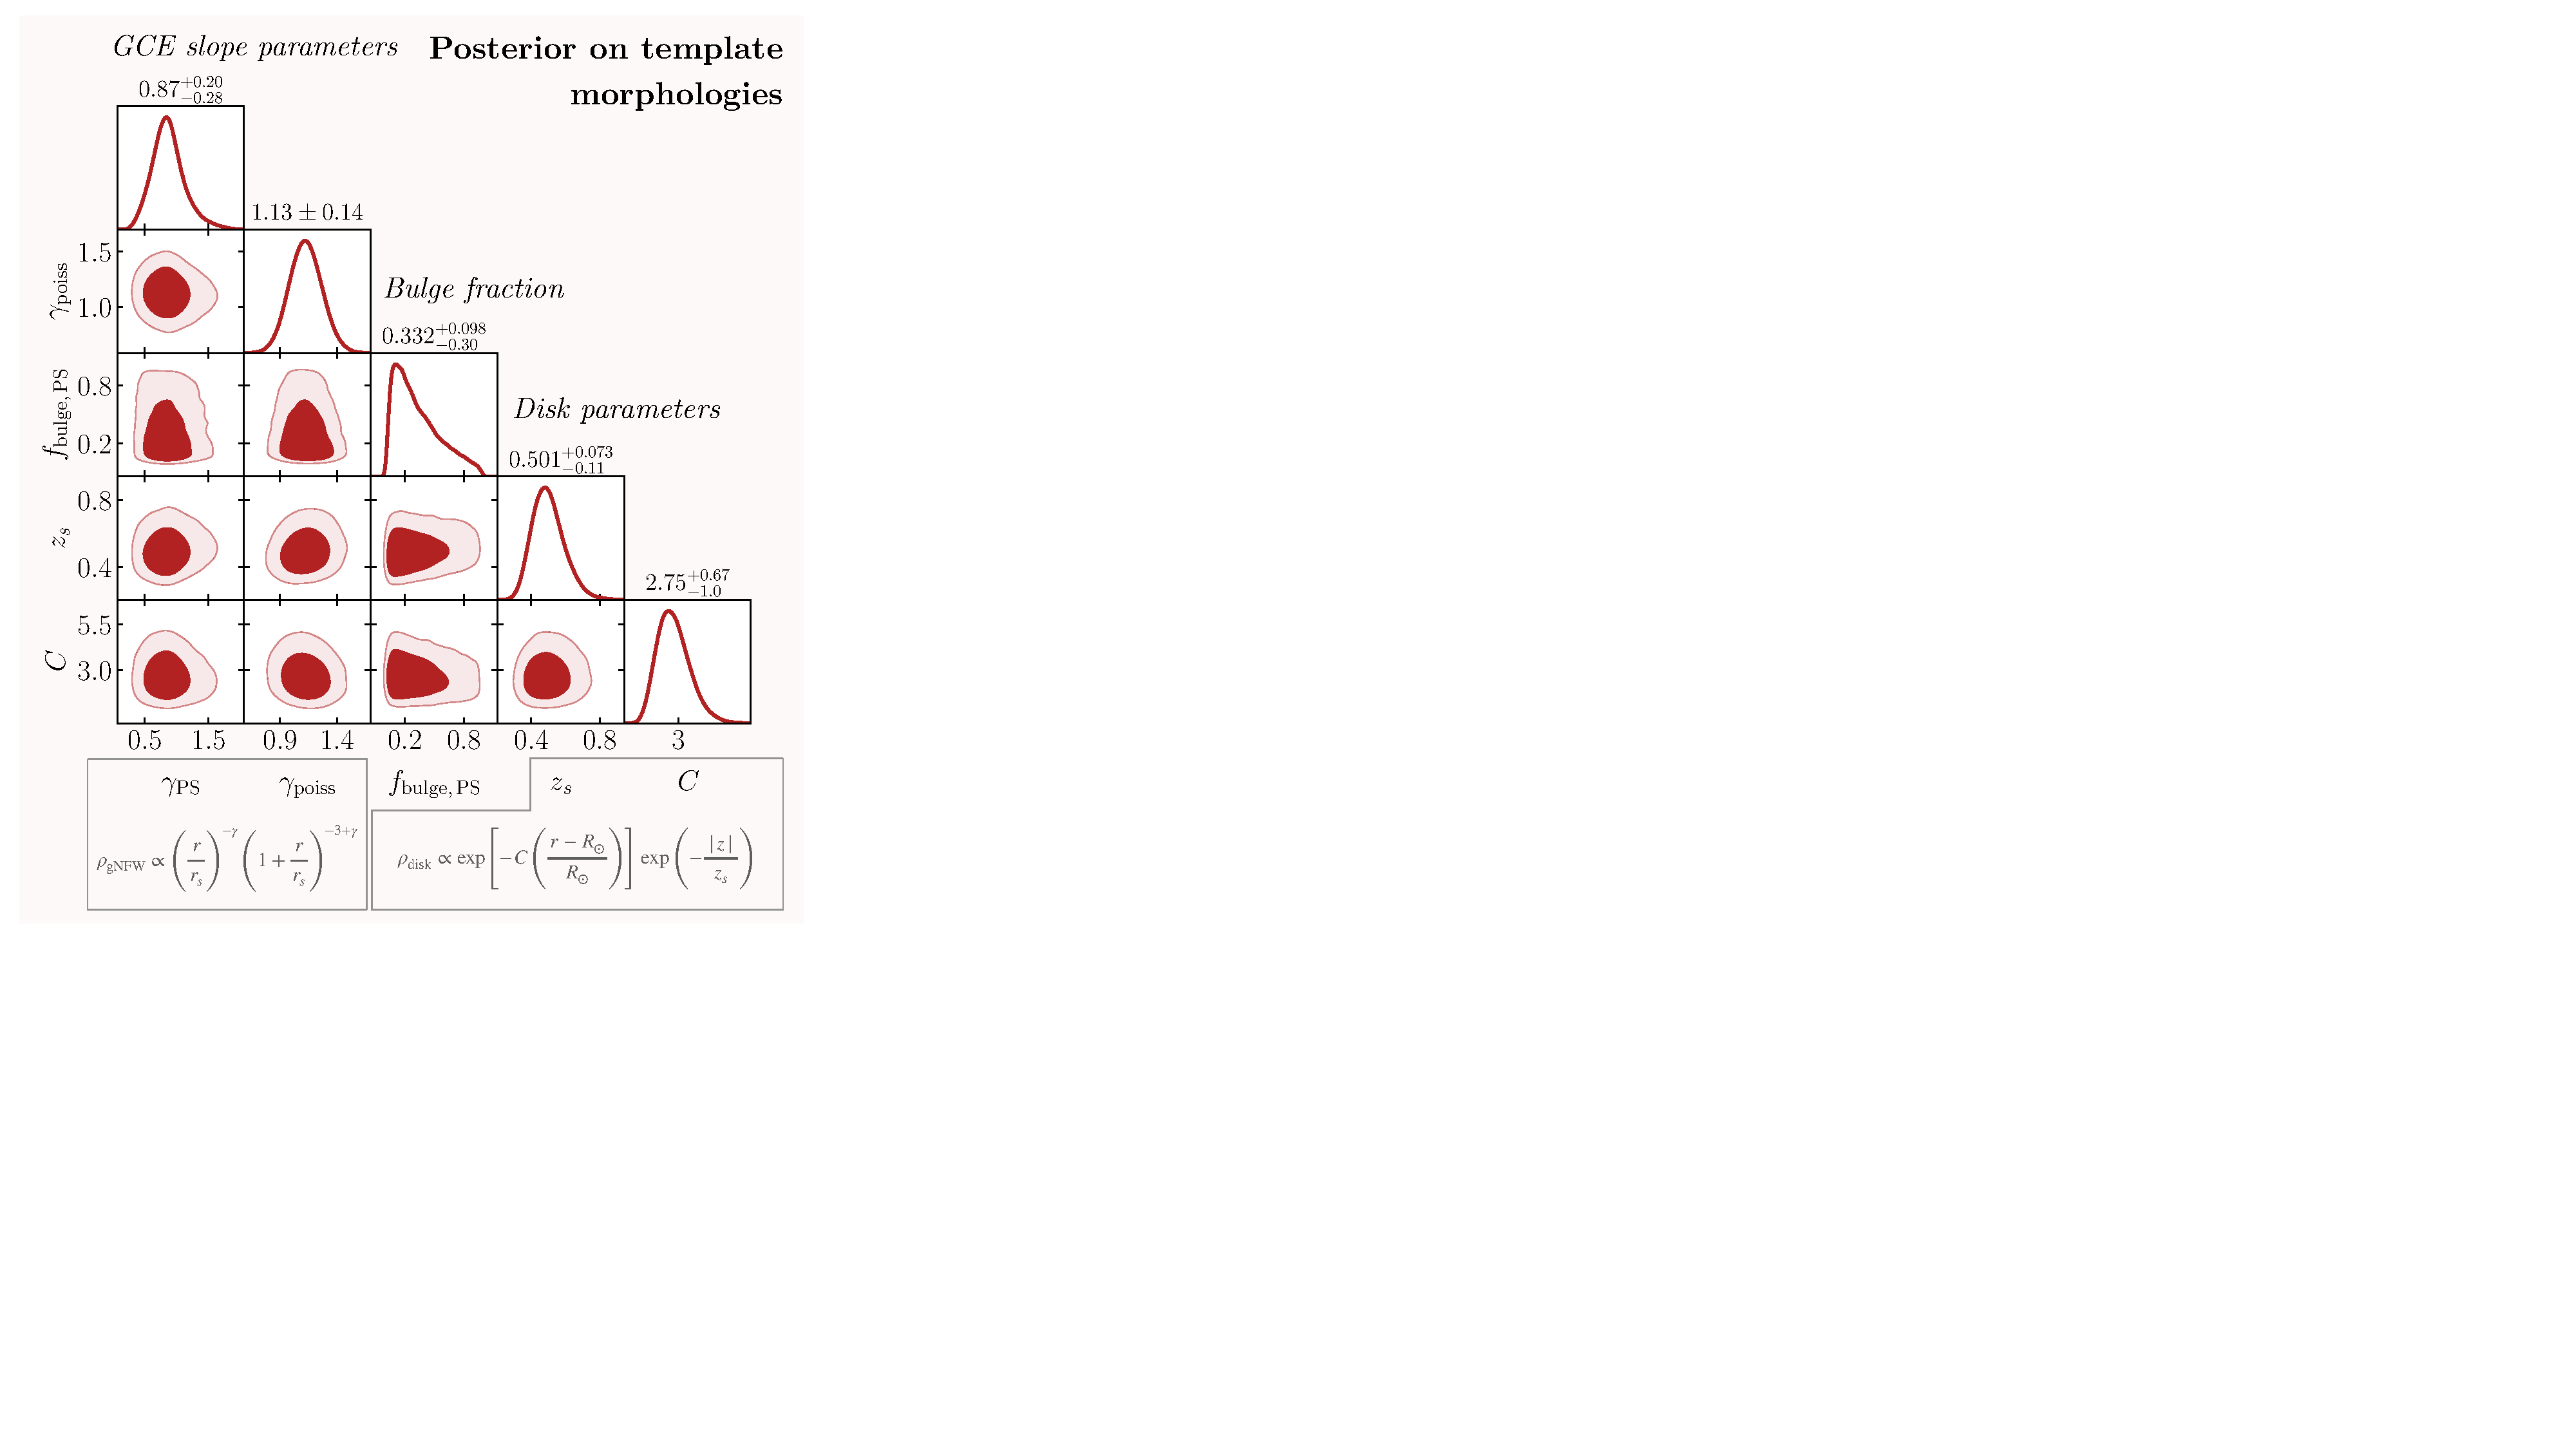
\includegraphics[width=0.48\textwidth]{figures/triangle.pdf}
\caption{\small{Subset of parameters describing the signal and disk morphologies from a preliminary fit on \Fermi data obtained using differentiable programming. Different panels display posteriors for the index $\gamma$ describing how the signal rises toward the Galactic Center, for PS and smooth components; the fraction of GCE-attributed PSs associated with the stellar bulge, $f_\mathrm{bulge}$; and the disk parameters $z_s$ and $C$. Expressions for profiles describing the GCE ($\rho_{\mathrm{gNFW}}$, generalized Navarro-Frenk-White, motivated by the DM hypothesis) as well as disk  ($\rho_\mathrm{disk}$, doubly-exponential) morphologies are shown.}}\vspace{-4mm}
\label{fig:figure}
\end{figure}

The entire pipeline will be end-to-end differentiable, meaning we can evaluate gradients of the log-likelihood function with respect to the parameters of interest $\theta$ characterizing the smooth as well as PS components, $\nabla_\theta\log\mathcal L(\theta)$. This opens up the possibility of using highly efficient gradient-based posterior inference techniques like Stochastic Variational Inference (SVI)~\cite{2012arXiv1206.7051H} and Hamiltonian Monte Carlo (HMC)~\cite{2011arXiv1111.4246H}. 
Unlike traditional sampling techniques employed in the context of \Fermi GCE analyses so far, these methods can easily scale up to high-dimensional parameter spaces. In particular, variational methods turn posterior inference into an optimization problem by fitting for a flexible functional ansatz on the posterior density and can easily deal with hundreds of parameters. This is in contrast to current public implementations of NPTF, which cannot efficiently include real-time generated templates at inference and are restricted to a modest $\lesssim30$ parameters with traditional Monte Carlo sampling techniques. We will release this code as an open-source package and make it available to the community for use in custom analyses.  %, following the precedent set by the original NPTF package co-developed by Co-I Mishra-Sharma.
% Concurrently, we will process and collect a large suite of diffuse foreground templates as well as templates describing possible spatial morphologies of the GCE from existing literature to be used in subsequent stages of the project. The Slatyer group has extensive prior experience with processing and analyzing \Fermi data~\cite{Daylan:2014rsa,Leane:2020nmi,Leane:2020pfc}. 
We will wrap the constructed likelihood using the probabilistic programming framework NumPyro~\cite{2019arXiv191211554P}, which allows for flexible specification of complex models as well as performing inference on them using gradient-based inference techniques. 
Illustrative results for the posterior on the GCE and disk template parameters using a preliminary version of the NPTF likelihood written in Jax are shown in Fig.~\ref{fig:figure}. The scalability of our implementation will also support inclusion of a wider range of templates for Inner Galaxy PS populations 
% (examples shown in Fig.~\ref{fig:figure}(c)) 
and Galactic diffuse emission, although the development of improved diffuse models is beyond the scope of this proposal.
%Taking advantage of the scalability of our implementation, we will consider multiple Galactic diffuse background templates simultaneously, allowing the model to explore the correlation structure in the space of diffuse models. Finally. we will validate the ability of the model to accurately characterize different components in the presence of systematic uncertainties by using simulated data. An example of the joint posterior over three different diffuse templates previously considered in the literature obtained using the preliminary differentiable version of NPTF is shown in Fig.~\ref{fig:figure}(b).
%\begin{wrapfigure}{l}{0.5\textwidth}
%  \begin{center}
%    \includegraphics[width=\textwidth]{figures/fig2.pdf}
%  \end{center}
%  \caption{Multiple signal templates, of astrophysical as well as DM origin, proposed in the literature. Our analysis will be able to characterize Inner Galaxy PS populations without relying on specific assumptions about their morphology.}
%\end{wrapfigure}

\vspace{0.05in}

% \emph{Stage 2.---}Having laid the groundwork for the project, we will wrap the constructed likelihood using the probabilistic programming framework NumPyro~\cite{2019arXiv191211554P}, which allows for flexible specification of complex models as well as performing inference on them. After validating the ability of the model to accurately characterize different components in the presence of systematic uncertainties using simulated data, we will condition various configurations of the model on real \emph{Fermi}-LAT data in order to robustly disentangle various emission components in the Galactic Center region without relying on rigid assumptions about signal and background morphologies. We will allow for the spatial distribution of the GCE to follow a \emph{composite hypothesis}, consisting of a linear combination of DM-motivated templates and those following astrophysically-motivated Galactic bulge templates (Fig.~\ref{fig:figure}(c)). Given the ability of our model to easily deal with hundreds of parameters, we will consider an augmented description of the Galactic diffuse background, which has so far been the source of large systematic uncertainties in GCE analyses, consisting of combinations of a large number of different physically-motivated templates with varying normalizations in different parts of the sky. An example of the joint posterior over three different diffuse templates obtained using the preliminary differentiable version of NPTF is shown in Fig.~\ref{fig:figure}(b).

% \vspace{0.05in}

% \begin{wrapfigure}{r}{0.5\textwidth}
%     \includegraphics[width=0.5\textwidth]{example-image-1x1}
%     \caption{A wrapped figure going nicely inside the text.}\label{wrap-fig:1}
%     \end{wrapfigure}     


\emph{Stage 2.---}At this stage, we will have laid the groundwork to characterize the emission in the Inner Galaxy region, accounting for a larger model space, in a fully probabilistic manner. Directly building on the work done so far, our next goal will be to characterize the $\gamma$-ray PS populations in the Galactic Center in a fully signal model-independent manner, by scanning over a space of spatial \emph{functions} on the sky map, as opposed to using parametric descriptions of signal templates. We will use Gaussian processes to place a prior over this function space, which will allow us to specify a scale on which we expect the morphology of the signal to vary, leaving the per-pixel normalizations otherwise free. The posteriors over both the smooth as well as unresolved PS population templates will provide an important cross check with the fixed-template descriptions used so far, and will, for the first time, deliver a model-independent characterization of the spatial population of unresolved PSs in the Inner Galaxy. A similar Gaussian process-based technique was successfully implemented in Ref.~\cite{Mishra-Sharma:2020kjb} to augment the morphology of the diffuse foreground template. The inclusion of flexible spatial templates in the pipeline is enabled by the highly efficient and differentiable version of the NPTF likelihood that we will develop as part of Stage 1.
%Next, we will consider several extensions and novel methodological developments that will further shed light on the nature of the GCE. 
%We will characterize the $\gamma$-ray PS populations in the Galactic Center in a fully signal model-independent manner by scanning over a space of spatial \emph{functions} on the sky map, as opposed to using parametric descriptions of signal templates. We will use Gaussian processes to place a prior over this function space, which will allow us to specify a scale on which we expect the morphology of the signal to vary, leaving the per-pixel normalizations otherwise free. The posteriors over both the smooth as well as unresolved PS population templates will provide an important cross check with the fixed-template descriptions used so far (examples shown in Fig.~\ref{fig:figure}(c)) and will, for the first time, deliver a model-independent characterization of the spatial population of unresolved PSs in the Inner Galaxy.
% Co-I Mishra-Sharma previously proposed using a similar method based on Gaussian processes to augment the diffuse foreground model template~\cite{Mishra-Sharma:2020kjb}.

\vspace{0.05in}

\begin{figure*}
    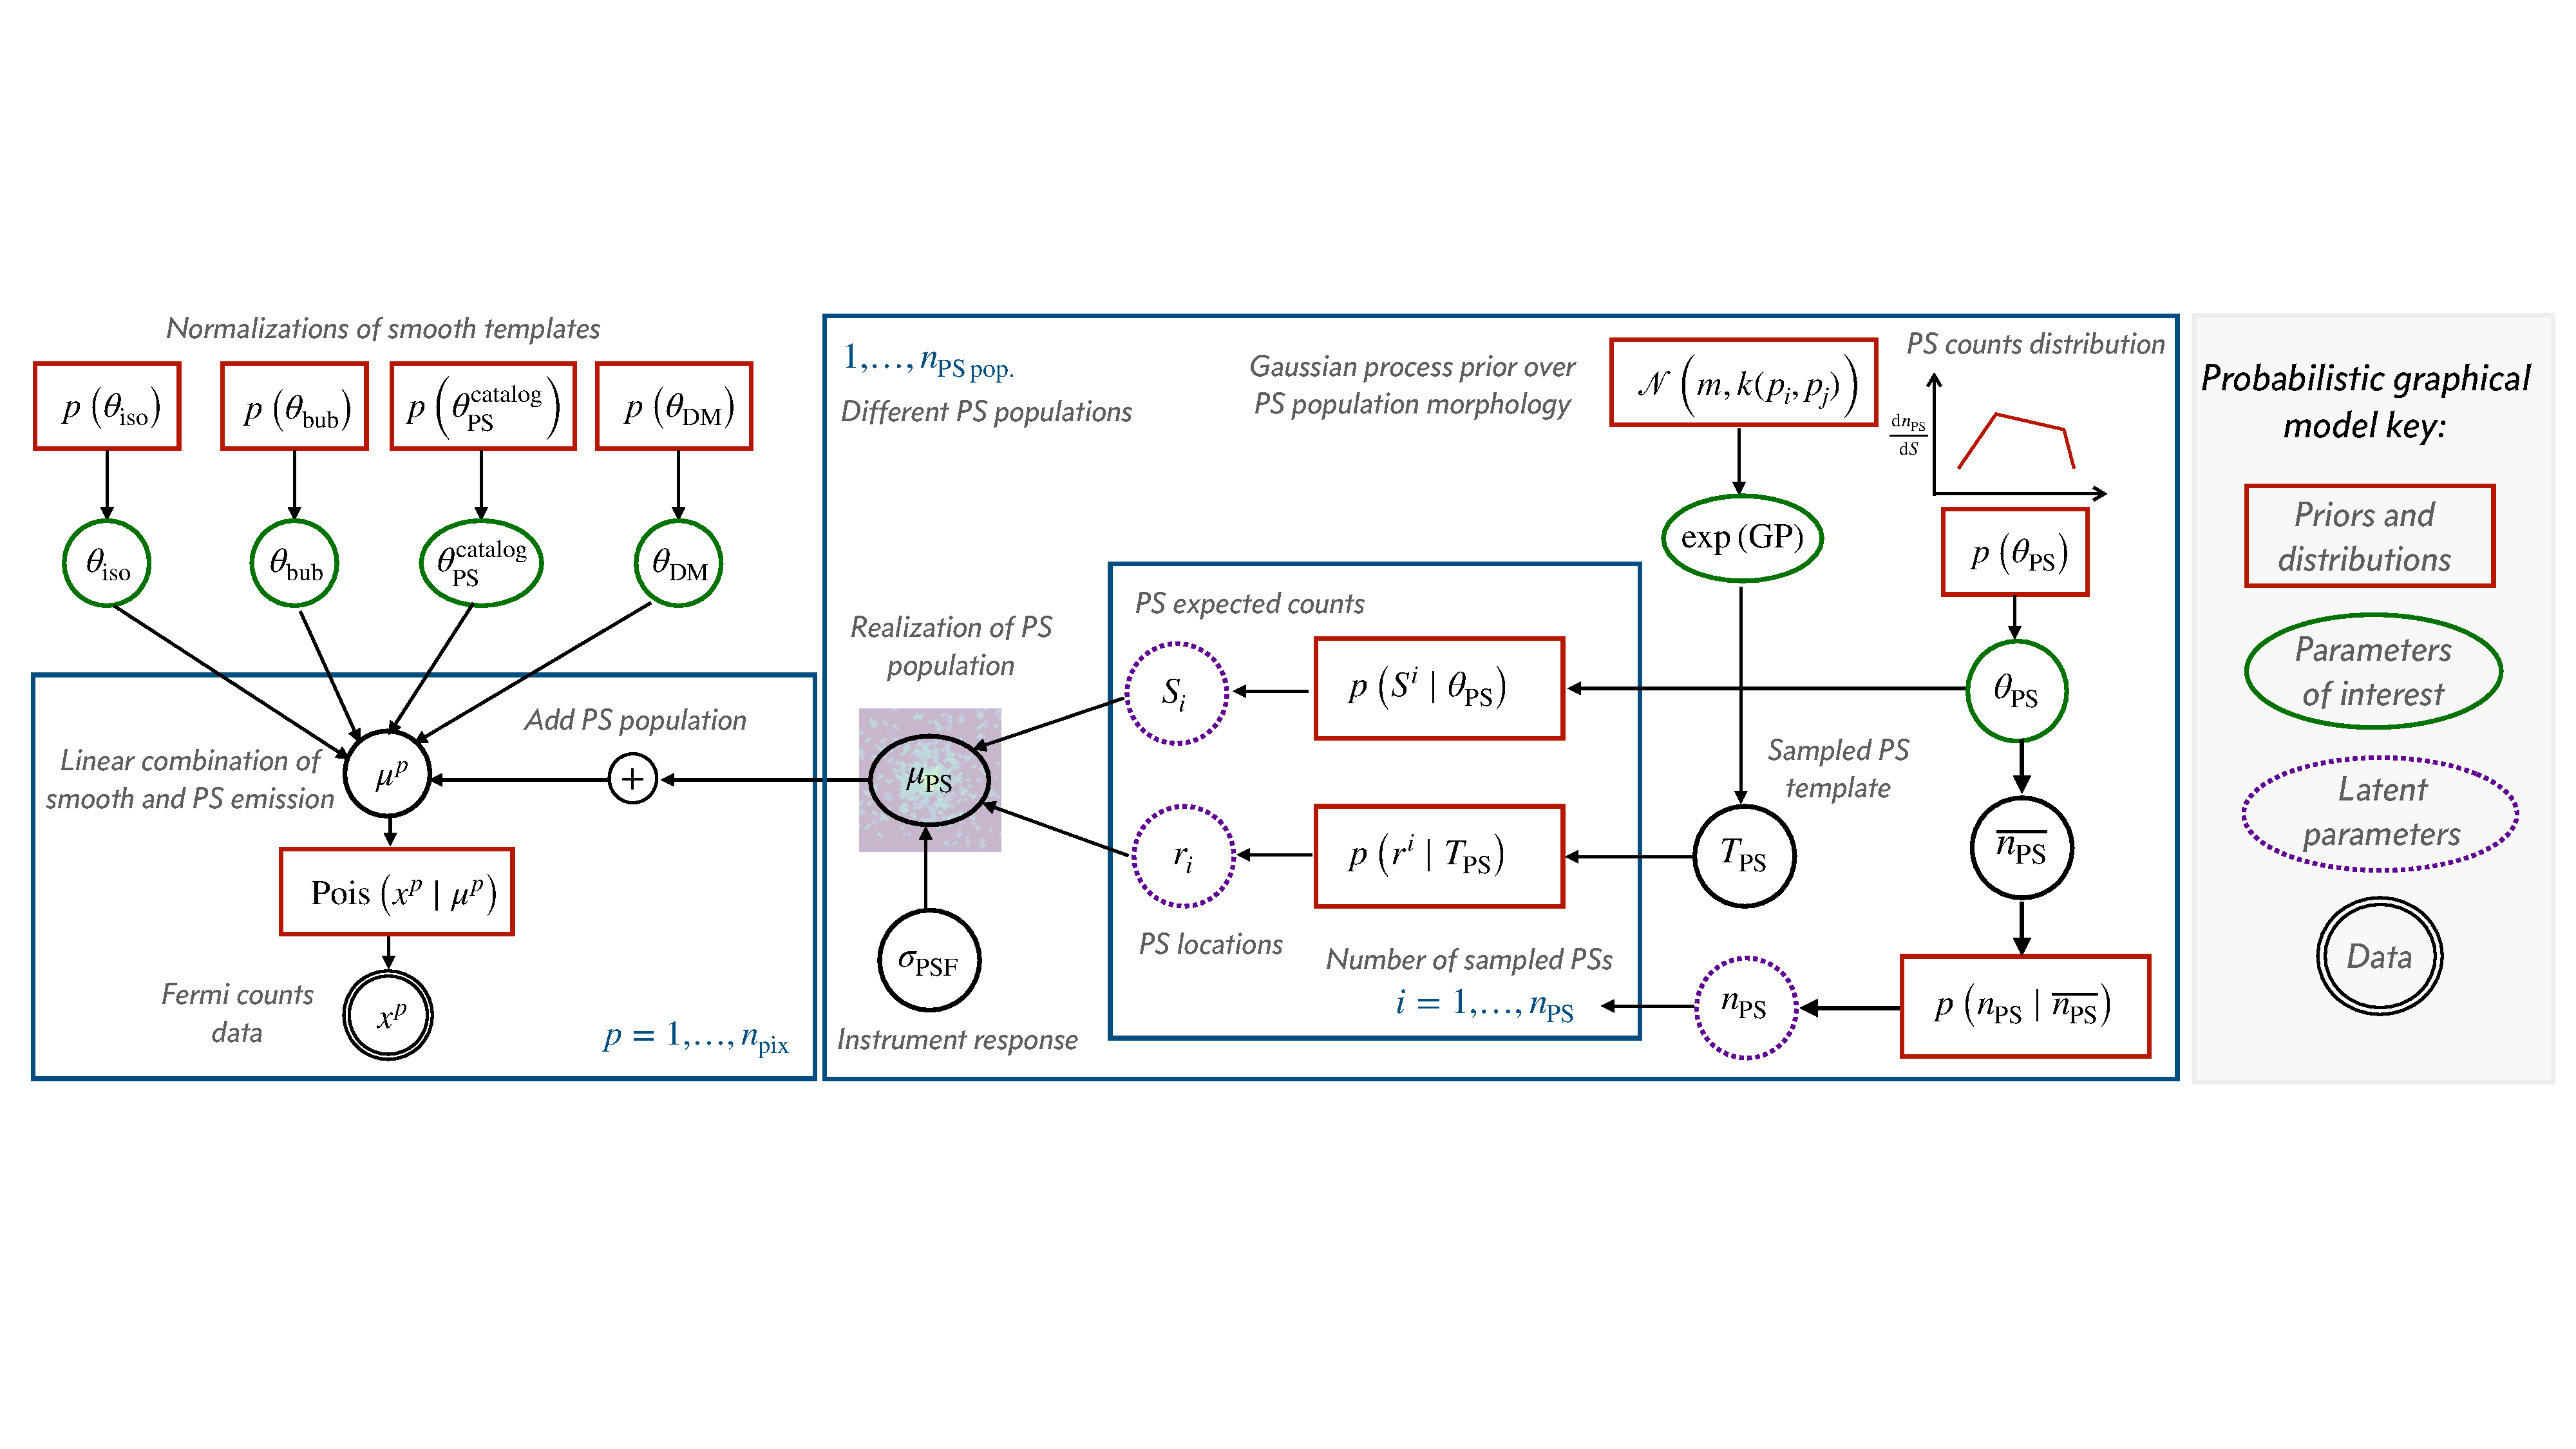
\includegraphics[width=0.97\textwidth]{figures/pgm.pdf}
    \caption{\small{Bayesian probabilistic graphical model (PGM) for a model of $\gamma$-ray emission in the Inner Galaxy region, including smooth emission (left side) and emission from unresolved PS populations (right side). For the smooth emission, normalizations of a spatially isotropic component ($\theta_\mathrm{iso}$), the \Fermi bubbles ($\theta_\mathrm{bub}$), resolved PSs ($\theta_\mathrm{PS}^\mathrm{catalog}$), and DM-like emission ($\theta_\mathrm{DM}$) are modeled. Distributions (including priors) are specified with red boxes, while random variables are specified with circles. Blue boxes indicate that the enclosed part of the model is independently repeated several times (over pixels, different PS populations, or individual PSs as specified). We will use the modern probabilistic programming framework NumPyro to implement this PGM and perform inference on it.}}
    \label{fig:pgm}
\end{figure*}
    
\emph{Stage 3.---}Non-Poissonian Template Fitting has been shown to be a powerful tool for characterizing PS populations in $\gamma$-ray data. However, the fact that the NPTF relies on a \emph{per-pixel} likelihood, which assumes each pixel to be conditionally independent, makes it demonstrably susceptible to model misspecification. 
The previous stages of this project have primarily focused on augmenting the plausible model-space, increasing the marginal probability that the NPTF likelihood encounters well-specified descriptions of the data. 
An orthogonal strategy involves innovating on the base method, and in particular implementing methods that can account for arbitrary inter-pixel correlation. Recent proposals in this direction involve the use of deep learning methods~\cite{2021PhRvD.104l3022L,2022PhRvD.105f3017M} and the construction of probabilistic catalogues with trans-dimensional sampling techniques~\cite{2017ApJ...839....4D}. 
For the final stage of this project, we will develop a complementary strategy that leverages recent developments in GPU-accelerated differentiable probabilistic programming that allow for automatic and efficient marginalization over large, discrete latent sites~\cite{2019arXiv190203210O,2023arXiv230200564L} -- in this case, the distribution of the number of unresolved PSs and their individual properties. An illustration of the Bayesian probabilistic graphical model (PGM) for the proposed model of Inner Galaxy $\gamma$-ray emission including smooth emission (left side) and different PS populations (right side) is shown in Fig.~\ref{fig:pgm}. 
% The NPTF likelihood implements this model while making several simplifying assumptions for computational feasibility. 
Modern probabilistic programming languages like NumPyro treat distributions (represented by red boxes in Fig.~\ref{fig:pgm}) and random variables (represented by circles in Fig.~\ref{fig:pgm}) as first-class objects, allowing for the specification of models in a manner that is syntactically close to the PGM. The model can then by directly used for performing inference (by conditioning it on observed data) as well as producing simulations (via sampling the model in the forward direction). The latter will be used to effectively validate the analysis results via posterior-predictive checks, which assess the compatibility between simulated realizations from the data-conditioned model and real data. Strategies such as \emph{enumeration}~\cite{2019arXiv190203210O}, which parallelize the likelihood computation over all possible combinations of the number of individual PSs, will be used to perform explicit marginalization while retaining the benefits of gradient-based posterior inference. This method will have several advantages over all existing approaches. Unlike the NPTF method, it will be able to fully account for pixel-to-pixel correlations. In contrast to machine learning-based approaches, being likelihood-based it will not require the use of black-box feature extractors, and additionally will easily scale to the larger model-spaces described in previous stages of the project since it will not rely on the use of pre-specified training data that is required to have support over the entire model-space.

\bibliography{fermi-prob-prog}
\bibliographystyle{icml2023}


%%%%%%%%%%%%%%%%%%%%%%%%%%%%%%%%%%%%%%%%%%%%%%%%%%%%%%%%%%%%%%%%%%%%%%%%%%%%%%%
%%%%%%%%%%%%%%%%%%%%%%%%%%%%%%%%%%%%%%%%%%%%%%%%%%%%%%%%%%%%%%%%%%%%%%%%%%%%%%%
% APPENDIX
%%%%%%%%%%%%%%%%%%%%%%%%%%%%%%%%%%%%%%%%%%%%%%%%%%%%%%%%%%%%%%%%%%%%%%%%%%%%%%%
%%%%%%%%%%%%%%%%%%%%%%%%%%%%%%%%%%%%%%%%%%%%%%%%%%%%%%%%%%%%%%%%%%%%%%%%%%%%%%%
\newpage
\appendix
\onecolumn
\section{You \emph{can} have an appendix here.}

You can have as much text here as you want. The main body must be at most $8$ pages long.
For the final version, one more page can be added.
If you want, you can use an appendix like this one, even using the one-column format.
%%%%%%%%%%%%%%%%%%%%%%%%%%%%%%%%%%%%%%%%%%%%%%%%%%%%%%%%%%%%%%%%%%%%%%%%%%%%%%%
%%%%%%%%%%%%%%%%%%%%%%%%%%%%%%%%%%%%%%%%%%%%%%%%%%%%%%%%%%%%%%%%%%%%%%%%%%%%%%%


\end{document}


% This document was modified from the file originally made available by
% Pat Langley and Andrea Danyluk for ICML-2K. This version was created
% by Iain Murray in 2018, and modified by Alexandre Bouchard in
% 2019 and 2021 and by Csaba Szepesvari, Gang Niu and Sivan Sabato in 2022.
% Modified again in 2023 by Sivan Sabato and Jonathan Scarlett.
% Previous contributors include Dan Roy, Lise Getoor and Tobias
% Scheffer, which was slightly modified from the 2010 version by
% Thorsten Joachims & Johannes Fuernkranz, slightly modified from the
% 2009 version by Kiri Wagstaff and Sam Roweis's 2008 version, which is
% slightly modified from Prasad Tadepalli's 2007 version which is a
% lightly changed version of the previous year's version by Andrew
% Moore, which was in turn edited from those of Kristian Kersting and
% Codrina Lauth. Alex Smola contributed to the algorithmic style files.
